\documentclass[11pt]{article}
\usepackage[utf8]{inputenc}
\usepackage{amsmath}
\usepackage{amssymb}
\usepackage{algpseudocode}
\usepackage{listings}
\usepackage{xcolor}
\usepackage{booktabs}
\usepackage{graphicx}
\usepackage{hyperref}
\usepackage{geometry}
\usepackage{titlesec}
\usepackage{enumitem}
\usepackage{booktabs}
\usepackage{forest}
\usepackage{tikz}
\usepackage{import} 
\usepackage{multirow}
\usepackage[ruled,vlined]{algorithm2e}
\usetikzlibrary{calc, positioning, arrows.meta}
\geometry{a4paper, margin=1in}
\titleformat{\section}{\large\bfseries}{\thesection}{1em}{}
\titleformat{\subsection}{\normalsize\bfseries}{\thesubsection}{1em}{}

\definecolor{codegreen}{rgb}{0,0.6,0}
\definecolor{codegray}{rgb}{0.5,0.5,0.5}
\definecolor{codepurple}{rgb}{0.58,0,0.82}
\definecolor{backcolour}{rgb}{0.95,0.95,0.92}

\lstset{
    language=C++,
    backgroundcolor=\color{backcolour},   
    commentstyle=\color{codegreen},
    keywordstyle=\color{magenta},
    numberstyle=\tiny\color{codegray},
    stringstyle=\color{codepurple},
    basicstyle=\ttfamily\footnotesize,
    breakatwhitespace=false,         
    breaklines=true,                 
    captionpos=b,                    
    keepspaces=true,                 
    numbers=left,                    
    numbersep=5pt,                  
    showspaces=false,                
    showstringspaces=false,
    showtabs=false,                  
    tabsize=4,
    frame=lines,
}

\begin{document}

\begin{center}
    \centering
    {\Huge \textbf{CSC3060 Project 5 Report}} \\[0.5cm]
    
    \textbf{Student Name} \quad Chaoyi, Sun \\[0.1cm]
    \textbf{Student ID} \quad 124090550 \\[1cm]
\end{center}

\section{Data Parallelism}

The \texttt{naive\_bitwise} performs a custom bit-mixing transformation on each pair of 8-bit integers. For input bytes \(A\) and \(B\), with constants \(L = \texttt{0x5A}\) and \(R = \texttt{0xC3}\):

\[
\begin{aligned}
\text{mixed0} &= \big((A \oplus B) \land L\big) \;\lor\; \big(\lnot(A \land B) \land \lnot L \big) \\
\text{mixed1} &= \big((A \lor B) \oplus R\big) \land \big((A \land B) \lor \lnot R\big) \;\oplus\; (A \oplus B) \\
\text{result} &= \text{mixed0} \oplus \text{mixed1}
\end{aligned}
\]

\noindent Since all bitwise operations are per-byte independent, we pack 8 consecutive \texttt{int8\_t} values into a \texttt{uint64\_t} and compute on all 8 bytes in parallel using standard bitwise operators. This achieves 8× data-level parallelism and reduces instruction count. The remaining bytes are handled with scalar computation.

\section{Branch Optimization}

We eliminate branches using the arithmetic identity:

\[
\max(x,0) = \frac{x + |x|}{2} = \begin{cases}
x, & x \ge 0 \\
0, & x < 0
\end{cases}
\]

\noindent This formulation replaces the branch with branchless operations, completely avoiding misprediction penalties. Additionally, 8-way loop unrolling reduces loop overhead and improves instruction-level parallelism.

\vspace{0.3em}

\noindent In practice, $\texttt{std::max(0, x)}$ is even faster as it compiles to a single $\texttt{MAXSS}$ instruction, achieving the same branchless behavior with fewer operations. However, we present $\frac{x + |x|}{2}$ here to clearly illustrate the arithmetic transformation that eliminates branches.

\section{Cache Optimization}
\subsection{Matrix Multiplication}

To mitigate cache misses, we apply \textbf{tiling} with a block size of $B = 256$. Tiling partitions the matrices into $256 \times 256$ submatrices. These active blocks fit comfortably within the fast L1/L2 cache hierarchy, maximizing data reuse before eviction. This theoretically reduces the cache miss complexity from $\mathcal{O}(n^3)$ to $\mathcal{O}\left(\frac{n^3}{B}\right)$. The computation is partitioned as:

\[
C_{ij} = \sum_{k=0}^{n-1} A_{ik} B_{kj} \quad \Rightarrow \quad
C_{IJ} = \sum_{K} A_{IK} \times B_{KJ}\text{, where $I, J, K$ denote the partitioned block indices}
\]

\noindent Within each block, we perform loop permutation, reordering the nested loops from the standard $i$-$j$-$k$ sequence to $i$-$k$-$j$. Because matrix multiplication relies on scalar addition and multiplication, which are mathematically associative and commutative, accumulating the partial sums in a different order strictly preserves the final result. 

\[
C_{ij} = \sum_{k} A_{ik} B_{kj} \quad \xrightarrow{\text{reordered as}} \quad C_{i, *} \mathrel{+}= \sum_{k} \Big( A_{ik} \times B_{k, *} \Big)
\]

\subsection{Trace Replay}

The baseline accesses \texttt{records[trace[i]]} with random indices, defeating hardware prefetching. Each access suffers a cache miss, causing the processor to stall on memory latency.

\vspace {0.3em}

\noindent The optimized implementation uses software prefetching via the
\texttt{\_\_builtin\_prefetch} intrinsic. The solution employs double prefetching with distance 64 and two future indices are prefetched simultaneously, keeping multiple memory requests in flight. This overlaps computation with memory access more effectively, reducing stall cycles. The distance of 64 is tuned to balance timely data arrival against cache pollution on the course server.

\section{Optimized Data Structure}
\subsection{Graph}

\noindent Converting the pointer-based adjacency list to CSR format stores all edges in a contiguous array \texttt{col\_idx} with \texttt{row\_ptr} marking node boundaries:

\[
\texttt{row\_ptr} = [0,\; d_0,\; d_0+d_1,\; \ldots,\; |E|], \qquad
\texttt{col\_idx} = [\text{neigh}(0),\; \text{neigh}(1),\; \ldots]
\]

\noindent Traversal for node \(u\) becomes a linear scan over \(\texttt{col\_idx}[\texttt{row\_ptr}[u]:\texttt{row\_ptr}[u+1]]\). This eliminates pointer chasing and enables hardware prefetchers to load future cache lines in advance, significantly reducing cache misses.

\vspace{0.3em}

\noindent These transformations replace random pointer chasing with predictable sequential access, significantly reducing cache misses.

\subsection{Filter Gradient}

The baseline stores each channel in a separate \texttt{std::vector<float>}, requiring nine independent arrays. Accessing all channels of a pixel involves nine scattered memory loads.

\vspace{0.3em}

\noindent The optimization packs the nine channel values into a single \texttt{struct}, stored contiguously in one \texttt{std::vector<Pixel>}. A pixel's channels now reside in consecutive memory, allowing a single load to bring all nine values into the cache. This reduces memory accesses from nine per pixel to one, significantly improving spatial locality and cache efficiency.

\section{Bit Manipulation}

The baseline Black-Scholes kernel calls \texttt{std::sqrt}, \texttt{std::log}, and \texttt{std::exp} for each option price. These standard library functions are accurate to 1 ULP but introduce unnecessary overhead, as the checker only requires a relative tolerance of $5\times10^{-3}$.

\vspace{0.3em}

\noindent The optimization replaces these functions with fast approximations using bit-level manipulation:
\begin{itemize}
    \item \textbf{Square root} Fast inverse square root with Newton iteration. The method first approximates the reciprocal square root $\frac{1}{\sqrt{x}}$ using integer bit operations on the floating-point representation, then obtains $\sqrt{x} = x \cdot \frac{1}{\sqrt{x}}$.
    \item \textbf{Exponential} Using the identity $e^x = (1 + \frac{x}{n})^{n}$ with $n=256$, the approximation is computed by repeated squaring.
\end{itemize}

\section{Sparse Matrix Optimization}

The baseline implementation repeatedly loads the same CSR indices and
values for each dense column, and accesses the dense matrix with a large
stride, causing frequent cache misses.

\vspace{0.3em}

\noindent The optimization applies two techniques. First, the loop order is
interchanged so that each non-zero element is loaded once and reused
across all dense columns. Second, the dense matrix is transposed from
$[\text{dense\_cols}][\text{cols}]$ to $[\text{cols}][\text{dense\_cols}]$,
turning strided accesses into sequential stream accesses and improving
cache efficiency.

\section{Loop Fusion}

\usetikzlibrary{arrows.meta}
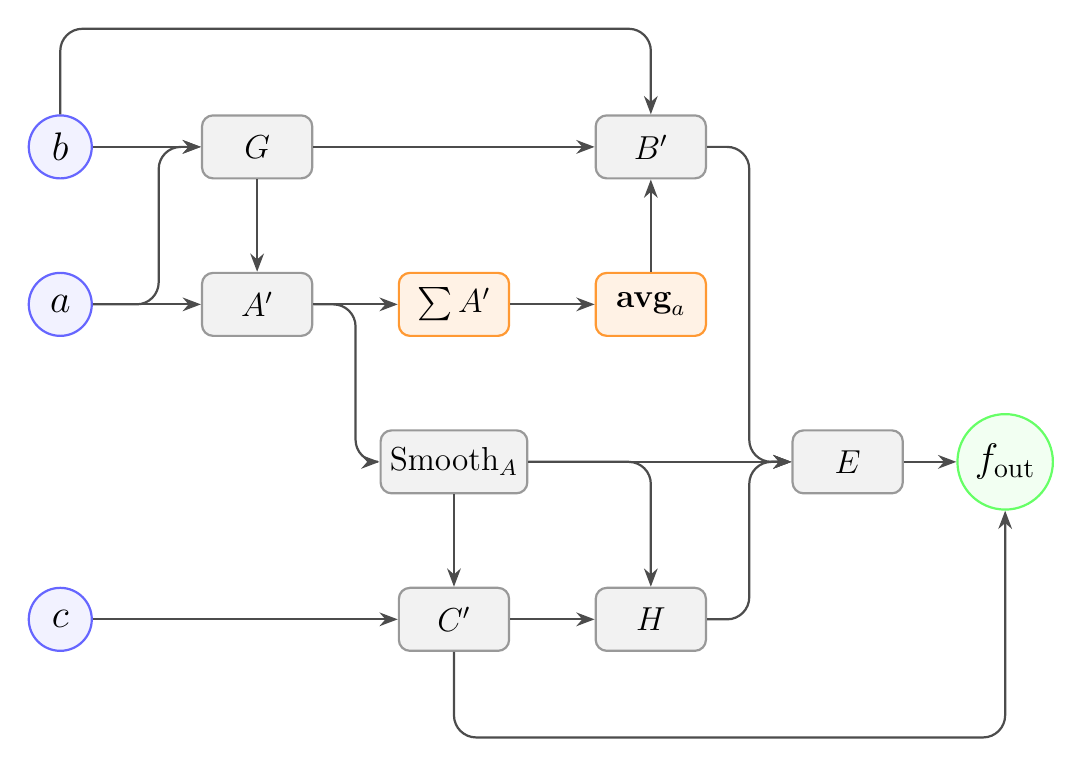
\begin{tikzpicture}[
    >=Stealth,
    % 统一定义节点样式
    input/.style={circle, draw=blue!60, fill=blue!5, thick, minimum size=8mm, font=\Large},
    output/.style={circle, draw=green!60, fill=green!5, thick, minimum size=8mm, font=\Large},
    op/.style={rectangle, draw=gray!80, fill=gray!10, thick, rounded corners, minimum width=1.4cm, minimum height=0.8cm, font=\large},
    global/.style={rectangle, draw=orange!80, fill=orange!10, thick, rounded corners, minimum width=1.4cm, minimum height=0.8cm, font=\large\bfseries},
    % 连线样式：加入 rounded corners=8pt 让正交拐角变得圆润、具有科技感
    edge/.style={->, thick, draw=black!70, rounded corners=8pt}
]

% ==================== 重新排列的绝对坐标网格 ====================

% 顶部计算流
\node[input] (b) at (0, 0) {$b$};
\node[op] (G) at (2.5, 0) {$G$};
\node[op] (Bprime) at (7.5, 0) {$B'$};

% 中上计算流 (同步层)
\node[input] (a) at (0, -2) {$a$};
\node[op] (Aprime) at (2.5, -2) {$A'$};
\node[global] (sum) at (5, -2) {$\sum A'$};
\node[global] (avg) at (7.5, -2) {$\text{avg}_a$};

% 中下计算流 (融合层)
\node[op] (Smooth) at (5, -4) {$\text{Smooth}_A$};
\node[op] (E) at (10, -4) {$E$};
\node[output] (out) at (12, -4) {$f_{\text{out}}$};

% 底部计算流
\node[input] (c) at (0, -6) {$c$};
\node[op] (Cprime) at (5, -6) {$C'$};
\node[op] (H) at (7.5, -6) {$H$};

% ==================== 智能正交连线 (零交叉) ====================

% 1. 到 G 和 A' 的基础输入 (左侧)
\draw[edge] (b) -- (G);
\draw[edge] (a) -- (Aprime);
\draw[edge] (a) -| (1.25, 0) -- (G); % a 到 G：向右半步，再向上，再平入
\draw[edge] (G) -- (Aprime);

% 2. 全局同步主线 (中间层)
\draw[edge] (Aprime) -- (sum);
\draw[edge] (sum) -- (avg);
\draw[edge] (avg) -- (Bprime);

% 3. 跨度较大的 B' 依赖 (避开下方节点)
\draw[edge] (G) -- (Bprime); % G 到 B'：平移，完美避让
\draw[edge] (b.north) |- (3.75, 1.5) -| (Bprime.north); % b 到 B'：从顶部上方绕行通道

% 4. Smooth_A 和 C' 的前置
\draw[edge] (Aprime) -| (3.75, -4) -- (Smooth); % A' 到 Smooth
\draw[edge] (c) -- (Cprime);
\draw[edge] (Smooth) -- (Cprime);

% 5. H 的计算
\draw[edge] (Cprime) -- (H);
\draw[edge] (Smooth) -| (H.north); % Smooth 到 H：向右合并后向下流入

% 6. E 的多路数据汇聚 (总线式合并)
\draw[edge] (Smooth) -- (E);
\draw[edge] (Bprime.east) -| (8.75, -4) -- (E); % 从上方降下，并入 -4 层总线
\draw[edge] (H.east) -| (8.75, -4) -- (E);      % 从下方升起，并入 -4 层总线

% 7. 最终输出
\draw[edge] (E) -- (out);
\draw[edge] (Cprime.south) |- (8.5, -7.5) -| (out.south); % C' 到 out：从底部下方绕行通道

\end{tikzpicture}

\noindent The baseline uses nine sequential loops, each writing intermediate results to memory and reloading them later, causing excessive memory traffic.

\vspace{0.3em}

\noindent The data dependencies show that $\text{avg}_a$ requires the sum of all $A'$, forcing at least two passes. The optimization restructures the computation into two passes:

\begin{itemize}
    \item Compute $A'$ and accumulate $\sum A'$.
    \item With $\text{avg}_a$ known, fuse Stages $4\sim 9$ into a single loop, keeping all intermediates in registers.
\end{itemize}

\section{Function Inline}

\subsection{Function Inlining}

The baseline calls seven functions per pixel, each with \texttt{noinline} attribute forcing call overhead and preventing cross-function optimizations.

\vspace{0.3em}

\noindent The optimization manually inlines small functions where call overhea dominates computation: \texttt{apply\_gain}, \texttt{apply\_shift}, \texttt{apply\_limit}, \texttt{color\_correct}, \texttt{compute\_gray}, \texttt{enhance\_contrast}, and \texttt{calculate\_gain}/\texttt{hdr\_compress}. Large functions with complex logic (\texttt{complex\_mask\_logic}, \texttt{importance\_weight}) remain as calls to avoid code bloat.

\vspace{0.3em}

\noindent This eliminates six function calls per pixel, enables constant propagation and common subexpression elimination, and allows the compiler to vectorize the inner loop.

\section{Bonus}

Use the parameters \(\texttt{-O3 -march=native -fno-associative-math}\)\\  \(\texttt{-fno-reciprocal-math -fno-trapping-math}\) in the \(\texttt{CMakeLists.txt}\). 

\begin{verbatim}
set_source_files_properties(
    ${CMAKE_SOURCE_DIR}/src/kernel/matmul.cpp
    PROPERTIES COMPILE_FLAGS "-O2 -fno-tree-vectorize"
)
\end{verbatim}

\noindent Also add the above to avoid floating-point precision discrepancies caused by compiler auto-vectorization. Since single-precision floating-point arithmetic is non-associative, altering the accumulation order via SIMD instructions leads to minor numerical deviations, which would trigger false positives in the strict relative error checker.

\vspace{0.3em}

\noindent To compensate for the performance penalty incurred by disabling SIMD vectorization, thread-level parallelism is introduced via OpenMP. Specifically, by applying the \texttt{\#pragma omp parallel for} directive to the outermost loop, the computational workload is distributed across multiple CPU cores. This allows independent matrix rows to be computed concurrently, achieving massive speedups without altering the strictly required thread-local accumulation order. To seamlessly integrate OpenMP at the build-system level, the following configuration is appended to the \(\texttt{CMakeLists.txt}\):

\begin{verbatim}
find_package(OpenMP REQUIRED)
target_link_libraries(kernels PUBLIC OpenMP::OpenMP_CXX)
\end{verbatim}

\section{Results}

\begin{table}[htbp]
    \centering
    \caption{Performance Comparison: Baseline vs. Basic vs. Bonus}
    \resizebox{\textwidth}{!}{
    \begin{tabular}{llrrrrr}
        \toprule
        \multirow{2}{*}{\textbf{Benchmark}} & \multirow{2}{*}{\textbf{Default Input Size}} & \multirow{2}{*}{\textbf{Baseline (ns)}} & \multicolumn{2}{c}{\textbf{Basic}} & \multicolumn{2}{c}{\textbf{Bonus}} \\
        \cmidrule(lr){4-5} \cmidrule(lr){6-7}
        & & & \textbf{Time (ns)} & \textbf{Speedup} & \textbf{Time (ns)} & \textbf{Speedup} \\
        \midrule
        Black-Scholes   & 81,920 options                            & 4,800,000   & 3,817,671  & 1.257x & 3,299,603  & 1.455x \\
        Sparse SpMM     & $2048 \times 2048$ for $S$ and $D^T$      & 116,000,000 & 79,345,670 & 1.462x & 55,047,604 & 2.107x \\
        ReLU            & vector length 1,024,000                   & 550,000     & 394,952    & 1.393x & 379,915    & 1.448x \\
        Bitwise         & vector length 1,024,000                   & 250,000     & 240,909    & 1.038x & 239,224    & 1.045x \\
        MatMul          & matrix size $512 \times 512$              & 88,000,000  & 77,836,484 & 1.131x & 47,984,715 & 1.834x \\
        Trace Replay    & 65,536 records, trace length 1,048,576    & 3,400,000   & 3,226,289  & 1.054x & 3,027,006  & 1.123x \\
        Graph           & 1,024,000 nodes, avg. degree 8            & 5,000,000   & 5,250,533  & 0.952x & 3,328,963  & 1.502x \\
        GRFF            & feature size 1,024,000                    & 8,500,000   & 8,855,230  & 0.960x & 3,312,860  & 2.566x \\
        Image Proc      & image size $1024 \times 1000$             & 43,000,000  & 42,494,877 & 1.012x & 1,916,674  & 22.435x \\
        Filter Gradient & $1024 \times 1024$ for height $\times$ width & 25,000,000 & 19,713,140 & 1.268x & 1,295,622  & 19.296x \\
        \midrule
        \textbf{Geometric Mean} & \textbf{-}                        & \textbf{-}  & \textbf{-} & \textbf{1.140x} & \textbf{-} & \textbf{2.632x} \\
        \bottomrule
    \end{tabular}
    }
\end{table}

\section{Appendix}

It is hereby declared that Generative AI tools were utilized in this project to assist with code optimization, report polishing, and test case generation. The core logic and implementation were verified by the author.
\end{document}